%% Do not edit unless you really know what you are doing.
\documentclass[english]{beamer}
\usepackage[T1]{fontenc}
\usepackage[latin9]{inputenc}
\setcounter{secnumdepth}{3}
\setcounter{tocdepth}{3}
\usepackage{amsfonts}
\usepackage{amssymb}
\usepackage{amsmath}
\usepackage{amsthm}
\usepackage{mathtools}
\usepackage{verbatim}
\usepackage{graphicx}
\usepackage{epstopdf}
\usepackage{amstext}
\usepackage{beamerthemesplit}
\usepackage{float}
\usepackage{tipa}
\usepackage{fancyhdr}
\usepackage{rotating}
\usepackage{natbib}
\usepackage{multicol}


\makeatletter
%%%%%%%%%%%%%%%%%%%%%%%%%%%%%% Textclass specific LaTeX commands.
 % this default might be overridden by plain title style
 \newcommand\makebeamertitle{\frame{\maketitle}}%
 \AtBeginDocument{
   \let\origtableofcontents=\tableofcontents
   \def\tableofcontents{\@ifnextchar[{\origtableofcontents}{\gobbletableofcontents}]}
   \def\gobbletableofcontents#1{\origtableofcontents}
 }

%%%%%%%%%%%%%%%%%%%%%%%%%%%%%% User specified LaTeX commands.


%\usepackage{beamerthemeshadow}

% Setting theme for presentation slides
\usetheme{Madrid} \usecolortheme{seahorse}
%\newcommand*\oldmacro{}
%\let\oldmacro\insertshorttitle % save previous definition
%\renewcommand*\insertshorttitle{
%\oldmacro \hfill  \leftskip=.2cm
%  \insertframenumber\,/\,\inserttotalframenumber}
\setbeamertemplate{footline}
{
  \leavevmode%
  \hbox{%
  \begin{beamercolorbox}[wd=.333333\paperwidth,ht=2.25ex,dp=1ex,center]{author in head/foot}%
    \usebeamerfont{author in head/foot}\insertsection
  \end{beamercolorbox}%
  \begin{beamercolorbox}[wd=.333333\paperwidth,ht=2.25ex,dp=1ex,center]{title in head/foot}%
    \usebeamerfont{title in head/foot}\insertsubsection
  \end{beamercolorbox}%
  \begin{beamercolorbox}[wd=.333333\paperwidth,ht=2.25ex,dp=1ex,right]{date in head/foot}%
    \usebeamerfont{date in head/foot}\insertshortdate{}\hspace*{2em}
    \insertframenumber{} / \inserttotalframenumber\hspace*{2ex} 
  \end{beamercolorbox}}%
  \vskip0pt%
}

\makeatother

\newcommand{\EEp}[1]{\mathbb{E}\left[#1\right]}


\newcommand{\bi}{\begin{itemize}[<+->]}
\newcommand{\ei}{\end{itemize}}
\newcommand{\eps}{\epsilon}
\newcommand{\nologo}{\setbeamertemplate{logo}{}} 

\begin{document}

\title{Deterministic Independent Component Analysis (ICA)}


\author{Ruitong Huang\hspace{4mm} Andr\'{a}s Gy\"{o}rgy \hspace{4mm}
 Csaba Szepesv\'ari}


\institute{University of Alberta}


\date{July 9, 2015 }
\logo{{\centering \includegraphics[width=5cm]{UA-CMPSCI-COLOUR.png} \hspace{0.5cm} \includegraphics[width=3cm]{logo.jpg}}\hspace{0.2cm}}

\makebeamertitle

\begin{frame}
\frametitle{Overview}
\tableofcontents 
\end{frame}

\section{Introduction}
\frame{ \frametitle{\, }
\centering
\LARGE What is ICA?
}

\frame{ \frametitle{Independent Component Analysis (ICA)} 
\bi 
\item A special case of Blind Source (Signal) Separation;
\onslide<+->
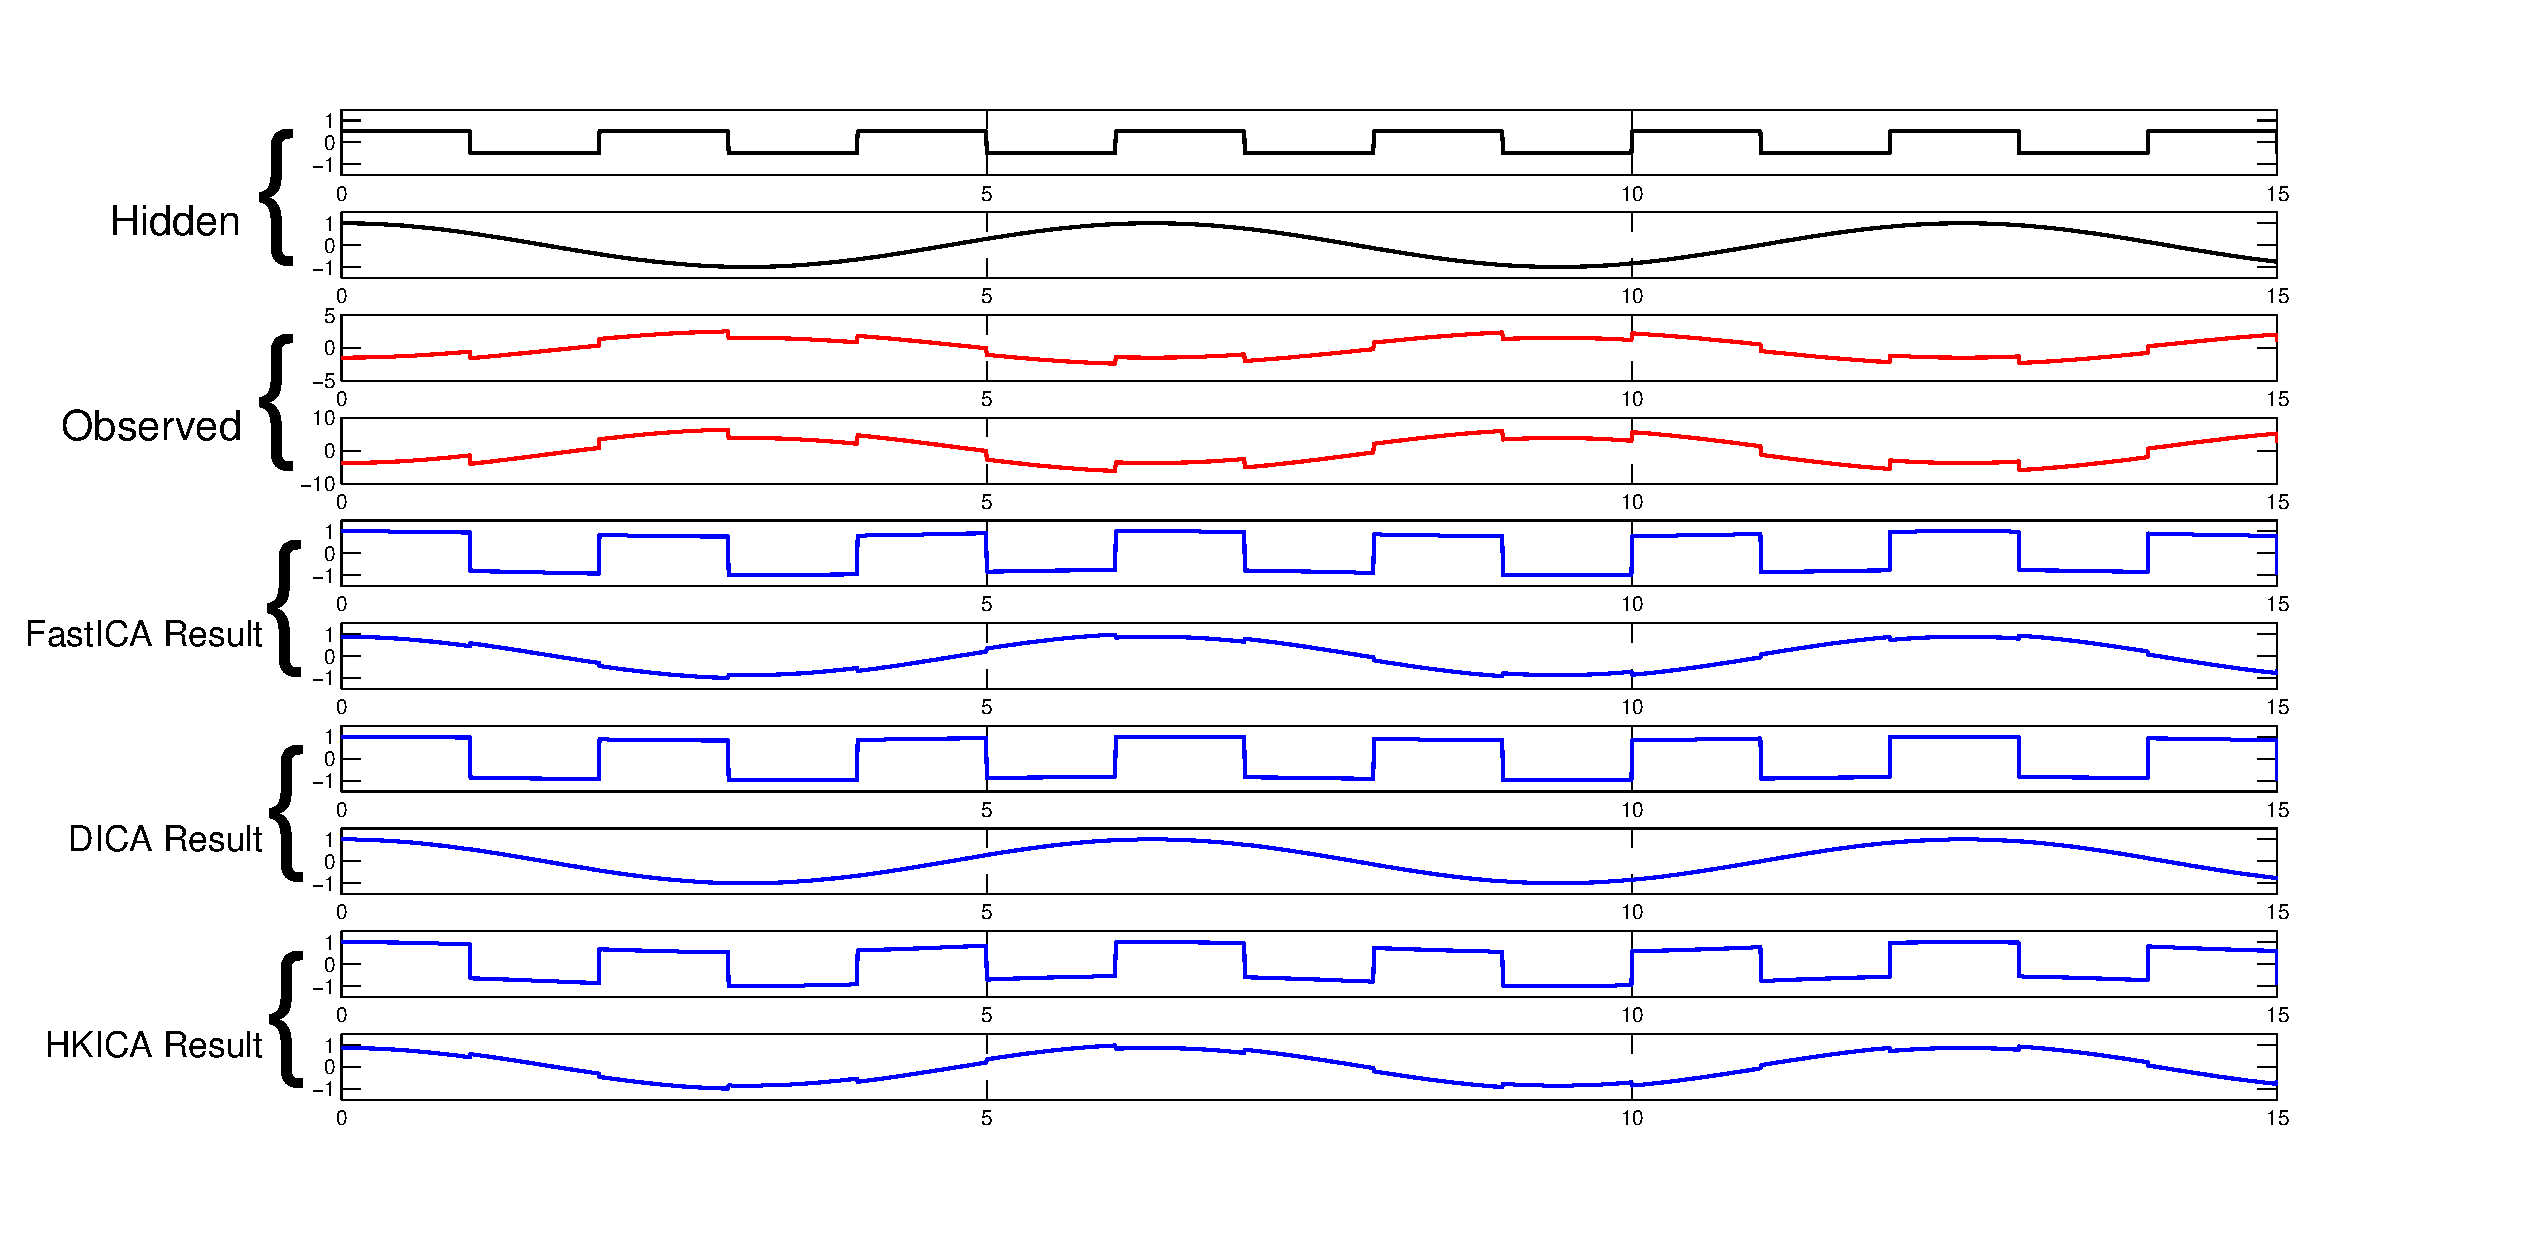
\includegraphics[width=.9\textwidth]{demo}
\ei
}

\frame{ \frametitle{Independent Component Analysis (ICA)} 
\bi 
\item  Model: $X = AS + \epsilon$; \\
\onslide<+->
\begin{center}
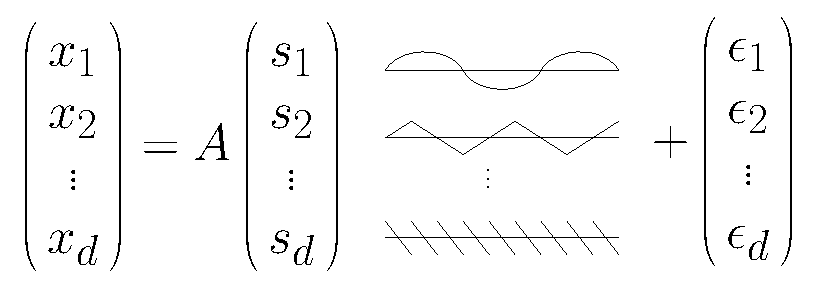
\includegraphics[width=8cm]{ICA_model.eps}
\end{center}
\item $S = (S_1,\ldots, S_d)$ non-Gaussian, $\eps \sim \mathcal{N}(0,\Sigma)$ Gaussian random variables.
\item Goal: Given $T$ independent observations $X(1), \ldots, X(T) \sim X$, reconstruct $A$ up to scaling and permutation. 
\ei
}
\frame{ \frametitle{Independent Component Analysis (ICA)} 
\begin{center}
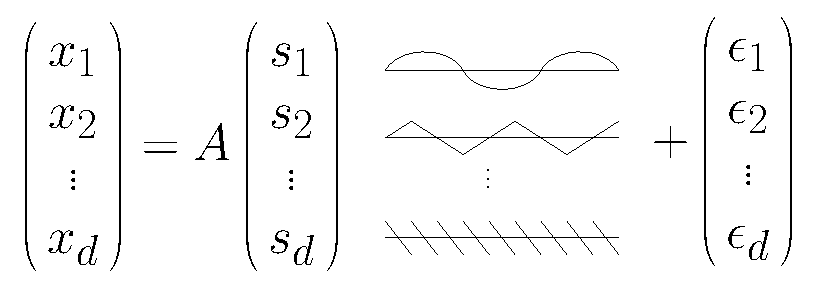
\includegraphics[width=8cm]{ICA_model.eps}
\end{center}
\bi
\item Assumptions:
	\bi
	\item[--] $S_1(t),\ldots, S_d(t)$, $\eps_1(t), \ldots, \eps_d(t)$ are mutually independent for any $t$.
	\vspace{0.3cm}
	\item[--] $A$ is non-singular (for simplicity). 
	\ei
\item Applications: Optical imaging; Telecommnications; Biology; Medicine. 
\ei
}

\frame{ \frametitle{Previous Works} 
Fast ICA {\scriptsize \citep{hyvarinen1999fast}};
\bi
\item Perhaps the most popular ICA algorithm.
\item With probability 1, all local optimizers are desired solutions \citep{wei2014study}, given:
	\begin{itemize}
	\item[--]<2-> infinitely many noiseless samples;
	\item[--]<2-> using kurtosis nonlinearity function.
	\end{itemize}
\item[-] In practice, its performance degrades for noisy periodic signals;
\ei

\onslide<+->
\vspace{1cm}
Moment methods were developed to avoid the local convergence problem; {\scriptsize\citep{DHsu2012, arora2012provable,goyal2014fourier}}
}

\frame{ \frametitle{Moment methods}
\bi
\item \citet{DHsu2012}'s method (HKICA); \\
\quad - No theoretical guarantee.
\item \citet{arora2012provable}'s method; \\
\quad - Free parameter.
\item Fourier PCA \citep{goyal2014fourier} (FPCA);\\
\quad - Free parameter.

\ei
}

\section{Our contributions}

\frame{ \frametitle{\, }
\centering
\LARGE Our Contributions
}

\frame{\frametitle{Our contributions}
\bi
\item It is well known that ICA works well on unmixing deterministic signals!
\item All deterministic sequences satisfy the independence assumption $\dots$
\item Can some ICA method unmix \alert{any} deterministic signals?
\ei
\bi
\item[$\diamondsuit$] Extend ICA to a non-stochastic setting that covers
	\begin{itemize}
	\item[--] the classic stochastic setting;
	\item[--] Markov sources;
	\item[--] deterministic source signals.
	\end{itemize}
\item[$\diamondsuit$] Develop, \emph{for the first time in the literature}, \alert{universal} ICA methods (i.e., no free parameters) that have
	\begin{itemize}
	\item[--] $\mathrm{poly}(T,d)$ runtime;
	\item[--] $\mathrm{lin}(D_4+1/\sqrt{T})$ accuracy (with i.i.d. noise). (the definition of $D_4$ will be introduced on the next slide.)
	\end{itemize}
\ei
}

\frame{ \frametitle{Result}
\bi
\item The source signals are a function of time: $s:[T] \to [-C,C]^d$.
\item Empirical distribution induced by function $s$:
	\[
	\nu_t^{(s)}(B)=\tfrac{1}{t}|\{\tau \in [t]: s(\tau) \in B\}|.
	\]
\item Independence measure of the sources:
	\[
	D_4	= \inf_{\mu} \sup_{f\in\mathcal{F}} \Big|\int f(s)d\nu_T^{(s)} - \int f(s)d\mu(s)\Big|,
	\]
	where $\mathcal{F}$ is the set of all monomials up to degree $4$
	and $\mu$ ranges over all product measures.
\ei
}

\frame{ \frametitle{Result (con't)}
There exist randomized methods to estimate $A$ from $x(t)=A s(t) + \eps(t)$, $t=1,\dots,T$ s.t.:
\bi
\item The computational complexity is $O(d^3 T)$;
\item With high probability there exists a permutation $\pi$ and 	constants $\{c_1,\ldots,c_d\}$, such that for all $1\le k\le d$, 
	\[
	\vert c_k\hat{A}_{\pi(k)} - A_k\vert_2 \le \theta_1 \min( D_4 + 1/\sqrt{T}, \theta_2 )\,.
	\]
\item Here, $\theta_1,\theta_2$ problem dependent, polynomial in the parameters.
\item  In the classical stochastic setting, $D_4= O(\frac{1}{\sqrt{T}})$.
\ei
}


\section{Deterministic ICA}
\frame{ \frametitle{\, }
\centering
\LARGE Deterministic ICA
}

\frame{ \frametitle{Hsu-Kakade method (HKICA)} 
\bi
\item[-] Let $f(\eta) = \EEp{(\eta^{\top}x)^4} - 3 \EEp{(\eta^{\top}x)^2}^2$;
\item[-] Choose $\phi$ and $\psi$. \emph{(How?)}
\item[-] Let $T(\phi) = \nabla^2 f(\phi)$. Then 
\[T(\phi) = AK 
\left(
\begin{array}{ccc}
\sigma_1 & & \\ 
    & \ddots & \\
    & & \sigma_d
\end{array} 
\right) 
A^{\top},
\]
where $\sigma_i = \left(\phi^{\top}A_i\right)^2$ and $K$ is some diagonal matrix.

\ei
}

\frame{ \frametitle{Hsu-Kakade method (HKICA)} 
\bi
\item[-] Let $M = T(\phi)(T(\psi))^{-1}$. Then 
\[M = A 
\left(
\begin{array}{ccc}
\lambda_1 & & \\ %\left(\frac{\phi^{\top}A_1}{\psi^{\top}A_1}\right)^2 & &\\
    & \ddots & \\
    & & \lambda_d %\left(\frac{\phi^{\top}A_d}{\psi^{\top}A_d}\right)^2\\
\end{array} 
\right) 
A^{-1},
\]
where $\lambda_i = \left(\frac{\phi^{\top}A_i}{\psi^{\top}A_i}\right)^2$.
\item[-] Do an eigen-decomposition of $M$ to recover $A$, assuming all $\lambda_i$'s are distinct.
\item[-] Given a finite sample, replace expectations with their empirical estimates.
\ei
}


\frame{ \frametitle{Issues with the HK method}
{\large{Problem: Minimal gap of the eigenvalues.}}			
\bi
\item Theoretical analysis shows that the performance depends on $\gamma_A^{-1}$, where
	\[
	\gamma_A = \min_{i\neq j} \left\vert \lambda_i - \lambda_j\right \vert.
	\]
\item $\gamma_A$ is not yet well understood
\item[] in particular, it is not known whether $\gamma_A^{-1} = \mathrm{Poly}(d,A)$\,.
\item Is this dependency of $\gamma_A^{-1}$ necessary?
\ei
}

\frame{ \frametitle{Our method: Deterministic ICA (DICA)}
\bi
\item[--] Inspired by \citet{arora2012provable} and \citet{frieze1996learning};
\item[--] Sample $\psi$, $\phi_1$ and $\phi_2$ independently from standard normal distribution.
\item[--] Calculate $\nabla^2 f(\psi)$ and $B$ such that $\nabla^2 f(\psi) = BB^{\top}$.
\item[--] Calculate $T(\phi_1) = \nabla^2 f(B^{-\top}\phi_1)$ and $T(\phi_2) = \nabla^2 f(B^{-\top}\phi_2)$.
\item Calculate $M = T(\phi_1)(T(\phi_2))^{-1}$.
	\[
	M = R \triangle\left( \tilde{\lambda}_1, \ldots, \tilde{\lambda}_d \right)R^{\top},
	\]
	where $\tilde{\lambda}_i = \left(\frac{\phi_1^{\top}R_i}{\phi_2^{\top}R_i}\right)^2$ and $R$ is some orthonormal matrix.
\item Do an eigen-decomposition of $M$ to recover $R$.
\item Return $\hat{A} = BR$ as an estimation of $A$. 
\ei
}

\frame{ \frametitle{Our method: Deterministic ICA (DICA)}
\bi
\item The reconstruction error is proportional to $\gamma_R^{-1}$, where 
	\[ 
	\gamma_R = \min_{i\neq j} \left\vert \tilde{\lambda}_i - \tilde{\lambda}_j\right \vert = \min_{i\neq j} \left\vert \left(\frac{\phi_1^{\top}R_i}{\phi_2^{\top}R_i}\right)^2
	 - \left(\frac{\phi_1^{\top}R_j}{\phi_2^{\top}R_j}\right)^2\right\vert.
	\]
	\bi
	\item[--] $\{\phi_1^{\top}R_1,\ldots, \phi_1^{\top}R_d, \phi_2^{\top}R_1,\ldots, \phi_2^{\top}R_d \}$ are independent standard normal variables.
	\item[--] No dependency on $A$.
	\item[--] Can be reduced to the minimal spacing of Cauchy random variables.
	\ei
\item Recursive version is also developed in the paper, based on the idea of \citet{vempala2014max}.
\ei
}

\section{Simulations}
\frame{ \frametitle{\, }
\centering
\LARGE Simulations
}

\frame{ \frametitle{Setting}
\vspace{-1cm}
\bi 
\item 9 different algorithms: 
	\bi
	\item<1-> HKICA (HKICA), and its recursive version (HKICA.R); 
	\item<1-> DICA  (DICA), and its recursive version (DICA.R); 
	\item<1-> A heuristic modification of  DICA  (MDICA), and its recursive version (MDICA.R);
	\item<1-> The default FastICA algorithm \citep{szabo12separation} (FICA);
	\item<1-> The recursive Fourier PCA \citep{vempala2014max}(FPCA);
	\item<1-> Random guessing (Random).
	\ei
\item 5 types of mixing matrices:
	\bi 
	\item<2-> $A = R$ is an orthonormal matrix;
	\item<2-> $A(A_1) = P$; 
	\item<2-> $A(A_2) = v_b\times\boldsymbol{1}' + 0.3\times P$;
	\item<2-> $A(A_3) = v_b\times\boldsymbol{1}' + 0.05\times P$;
	\item<2-> $A(A_4) = v_b\times\boldsymbol{1}' + 0.005\times P$  
	\item The vector $v_b$ and the matrix $P$ are both generated from standard normal distribution, and then normalized.
	\ei
\ei
}

\frame{ \frametitle{Setting}
\bi
\item 6-dimensional BPSK signals with different periods;
\item $x = As + c\eps$ for different noise ratio coefficients $c$;
\item $T = 20000$ observations;
\item Results are evaluated on a 150 repetitions. For each repetition, we try 3 times and report the best.
\ei
}

{\nologo
\frame{ \frametitle{Simulation resutls}
\begin{multicols}{3}
	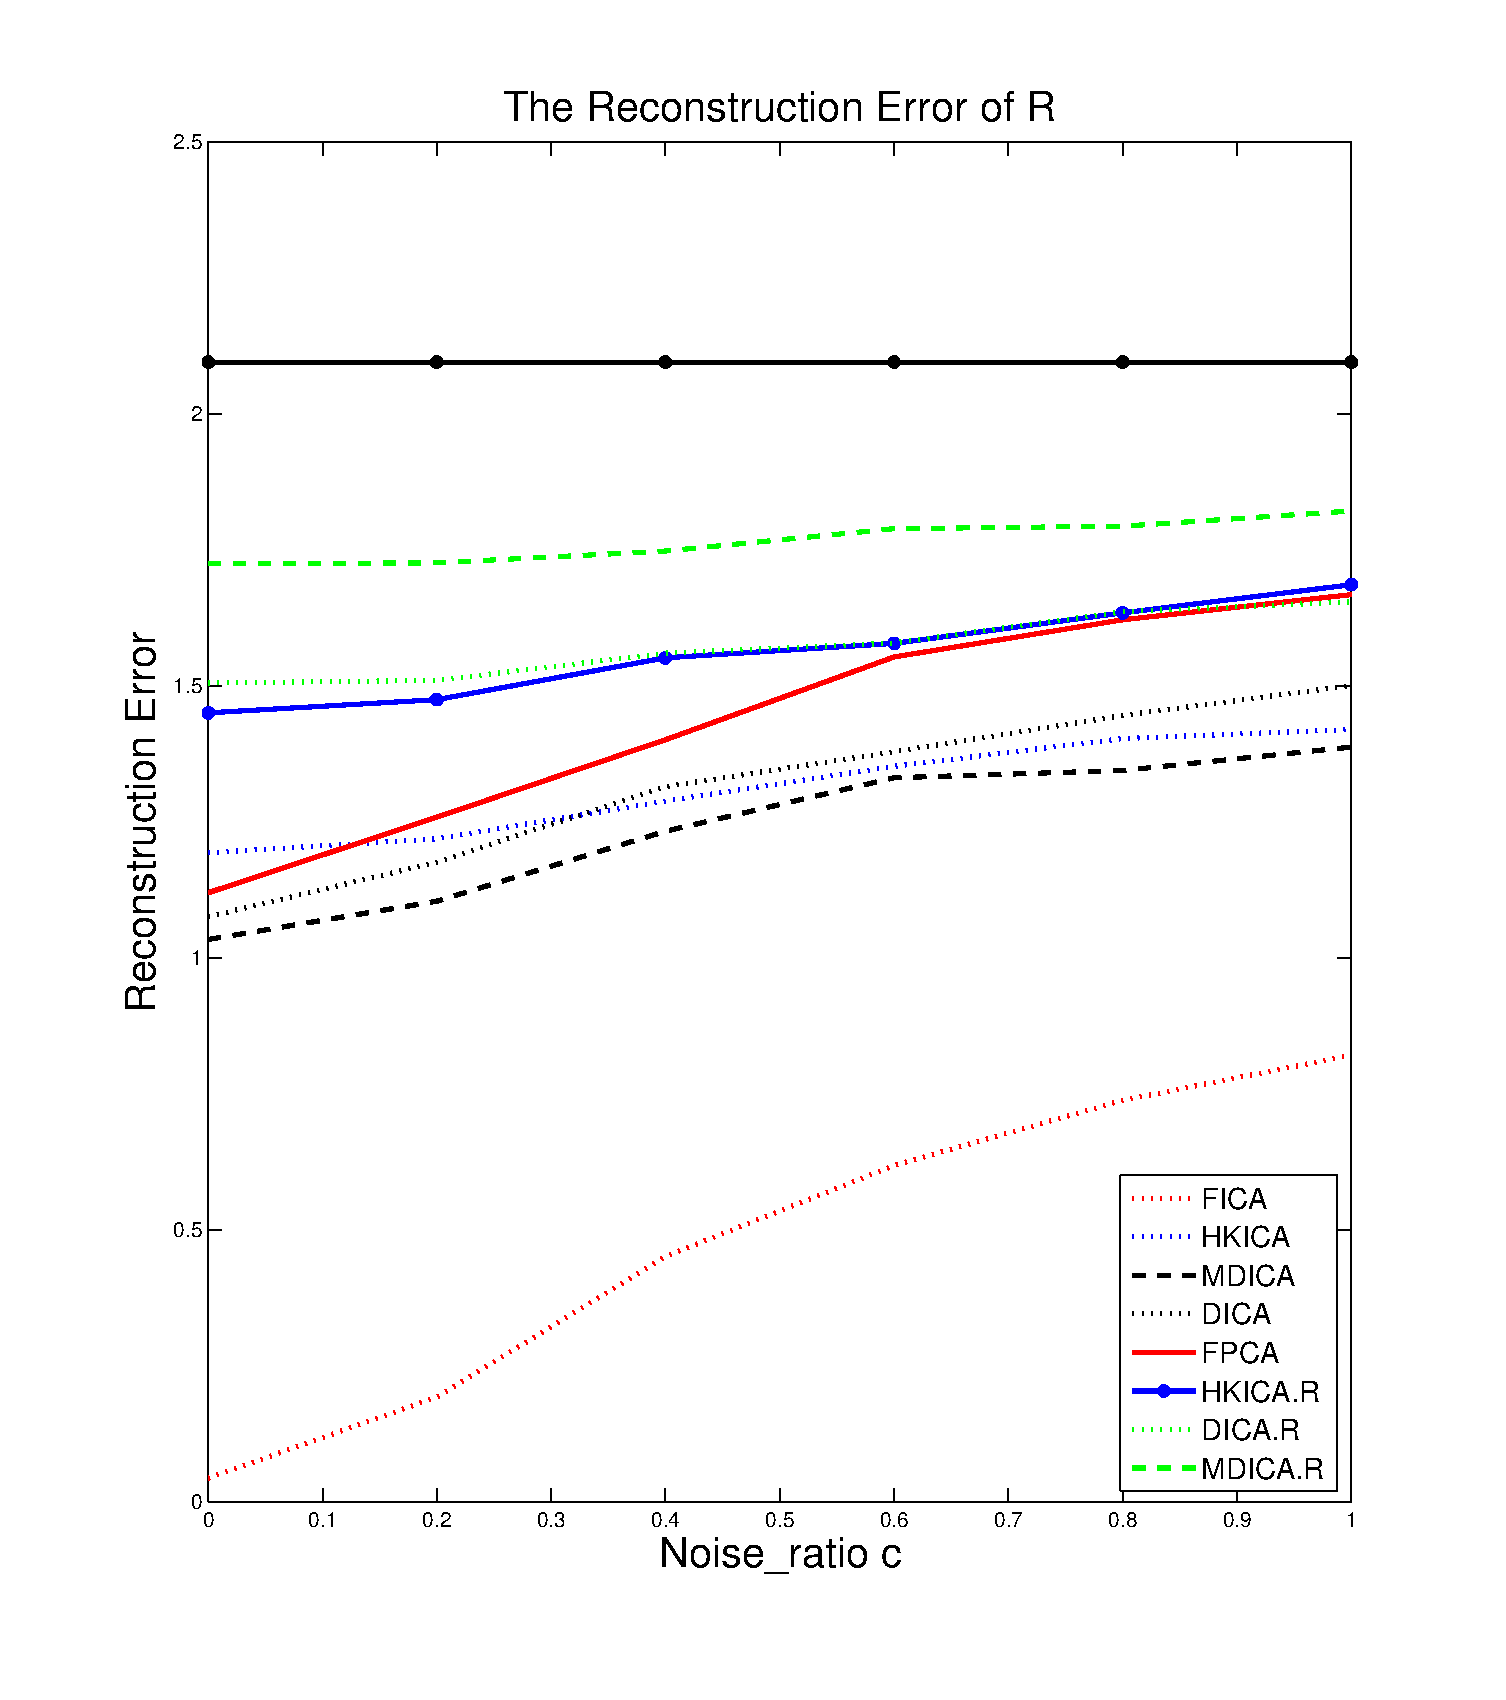
\includegraphics[height = 0.42\textheight]{errorR}\\
	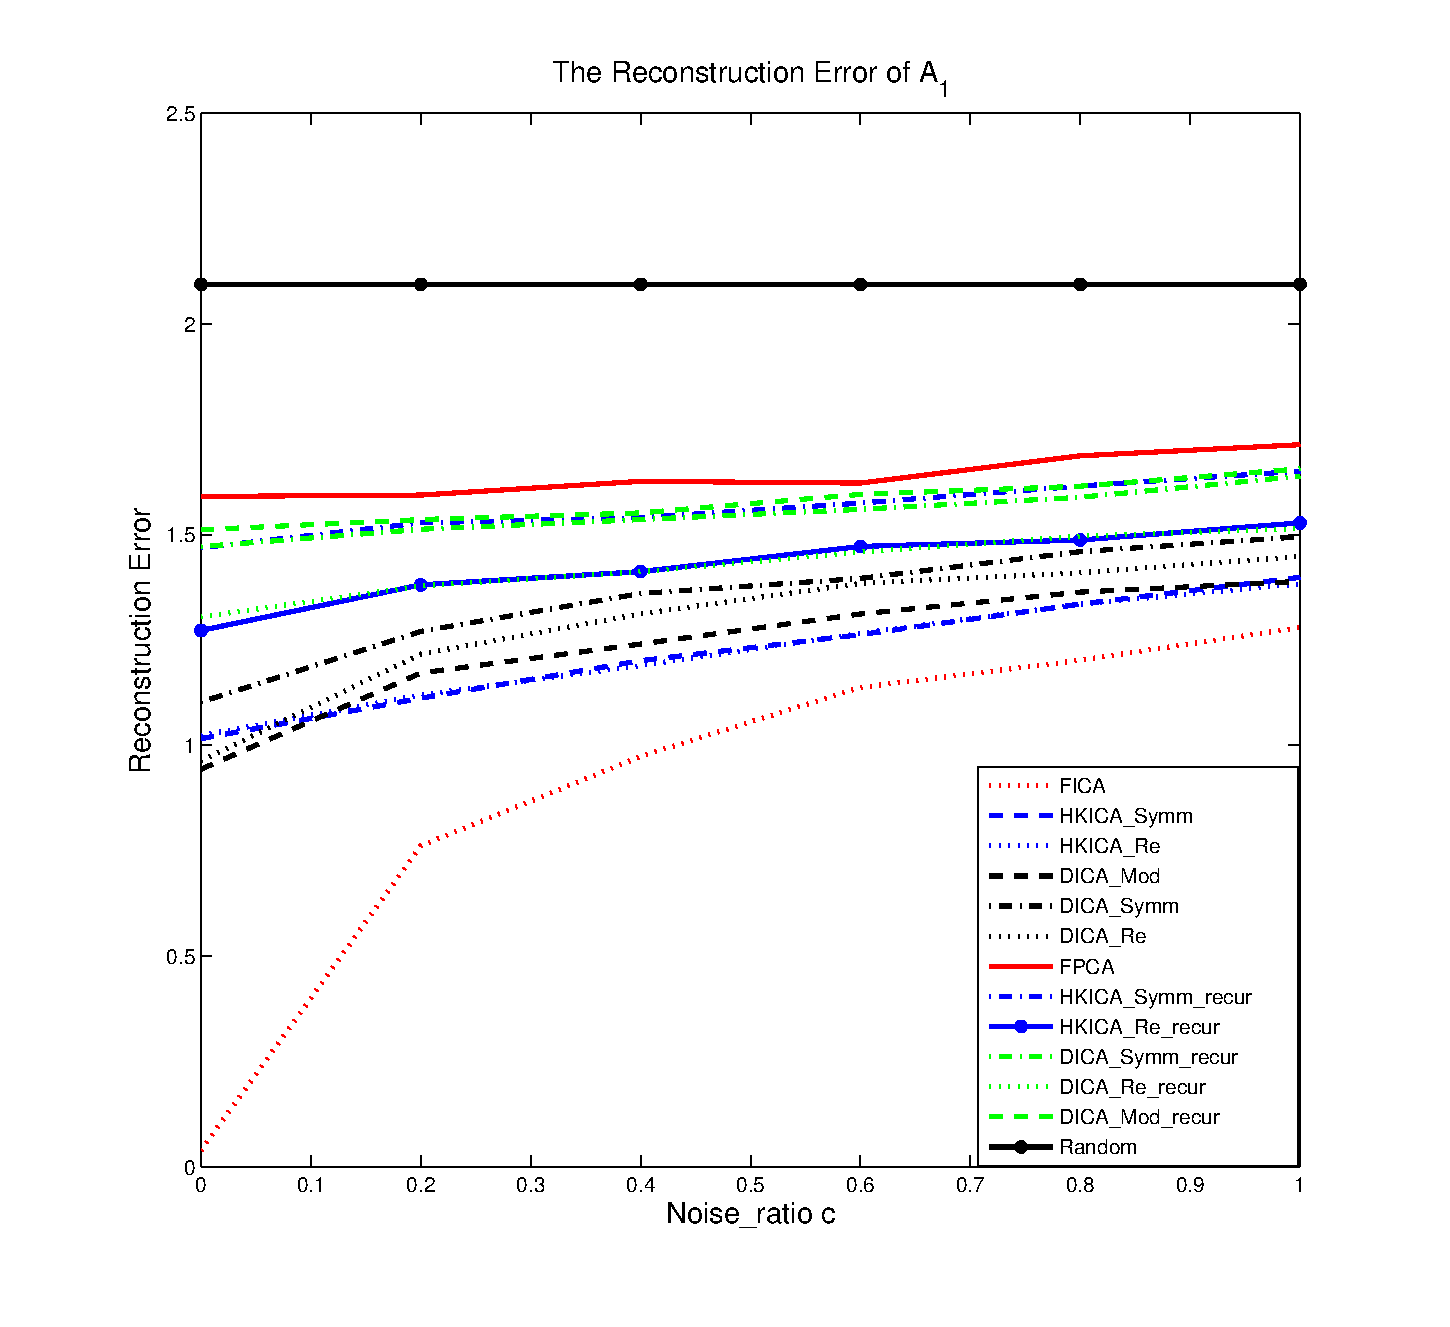
\includegraphics[height = 0.42\textheight]{error1}
	\newpage
	\topskip0pt
	\vspace*{\fill}
	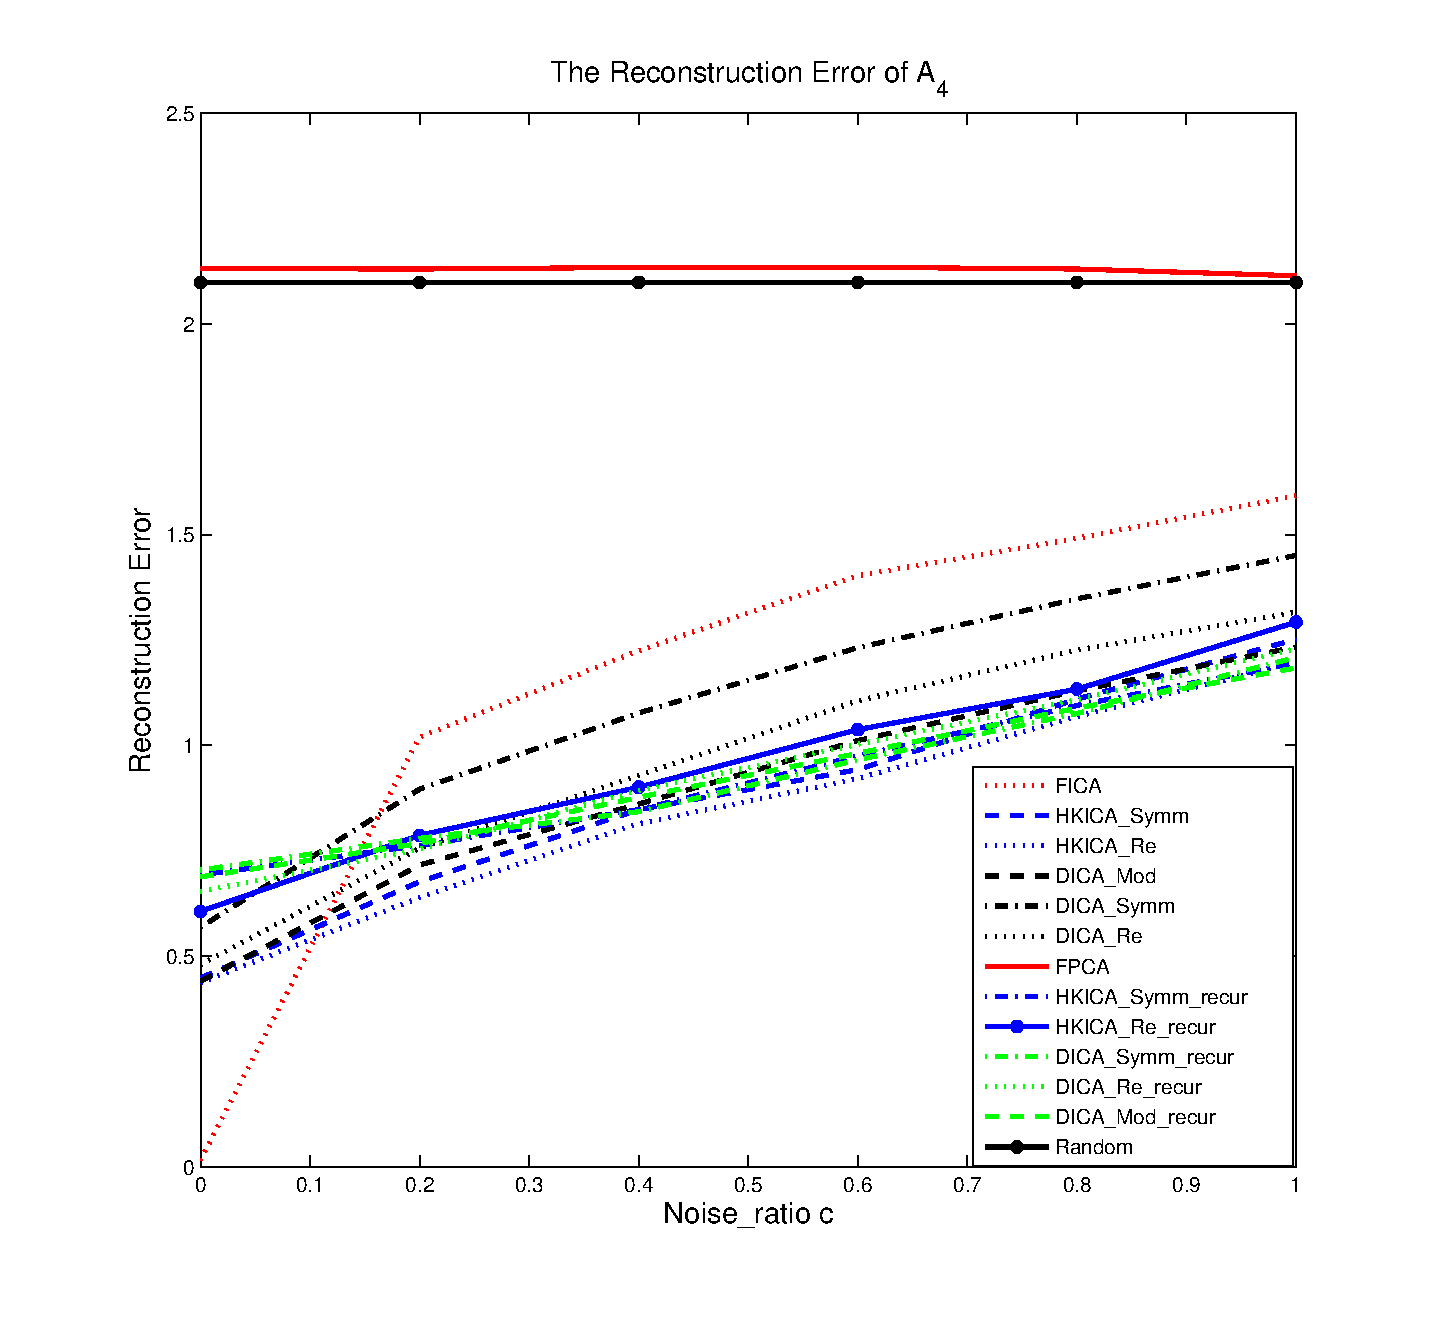
\includegraphics[height = 0.42\textheight]{error2}
	\vspace*{\fill}
	\newpage
	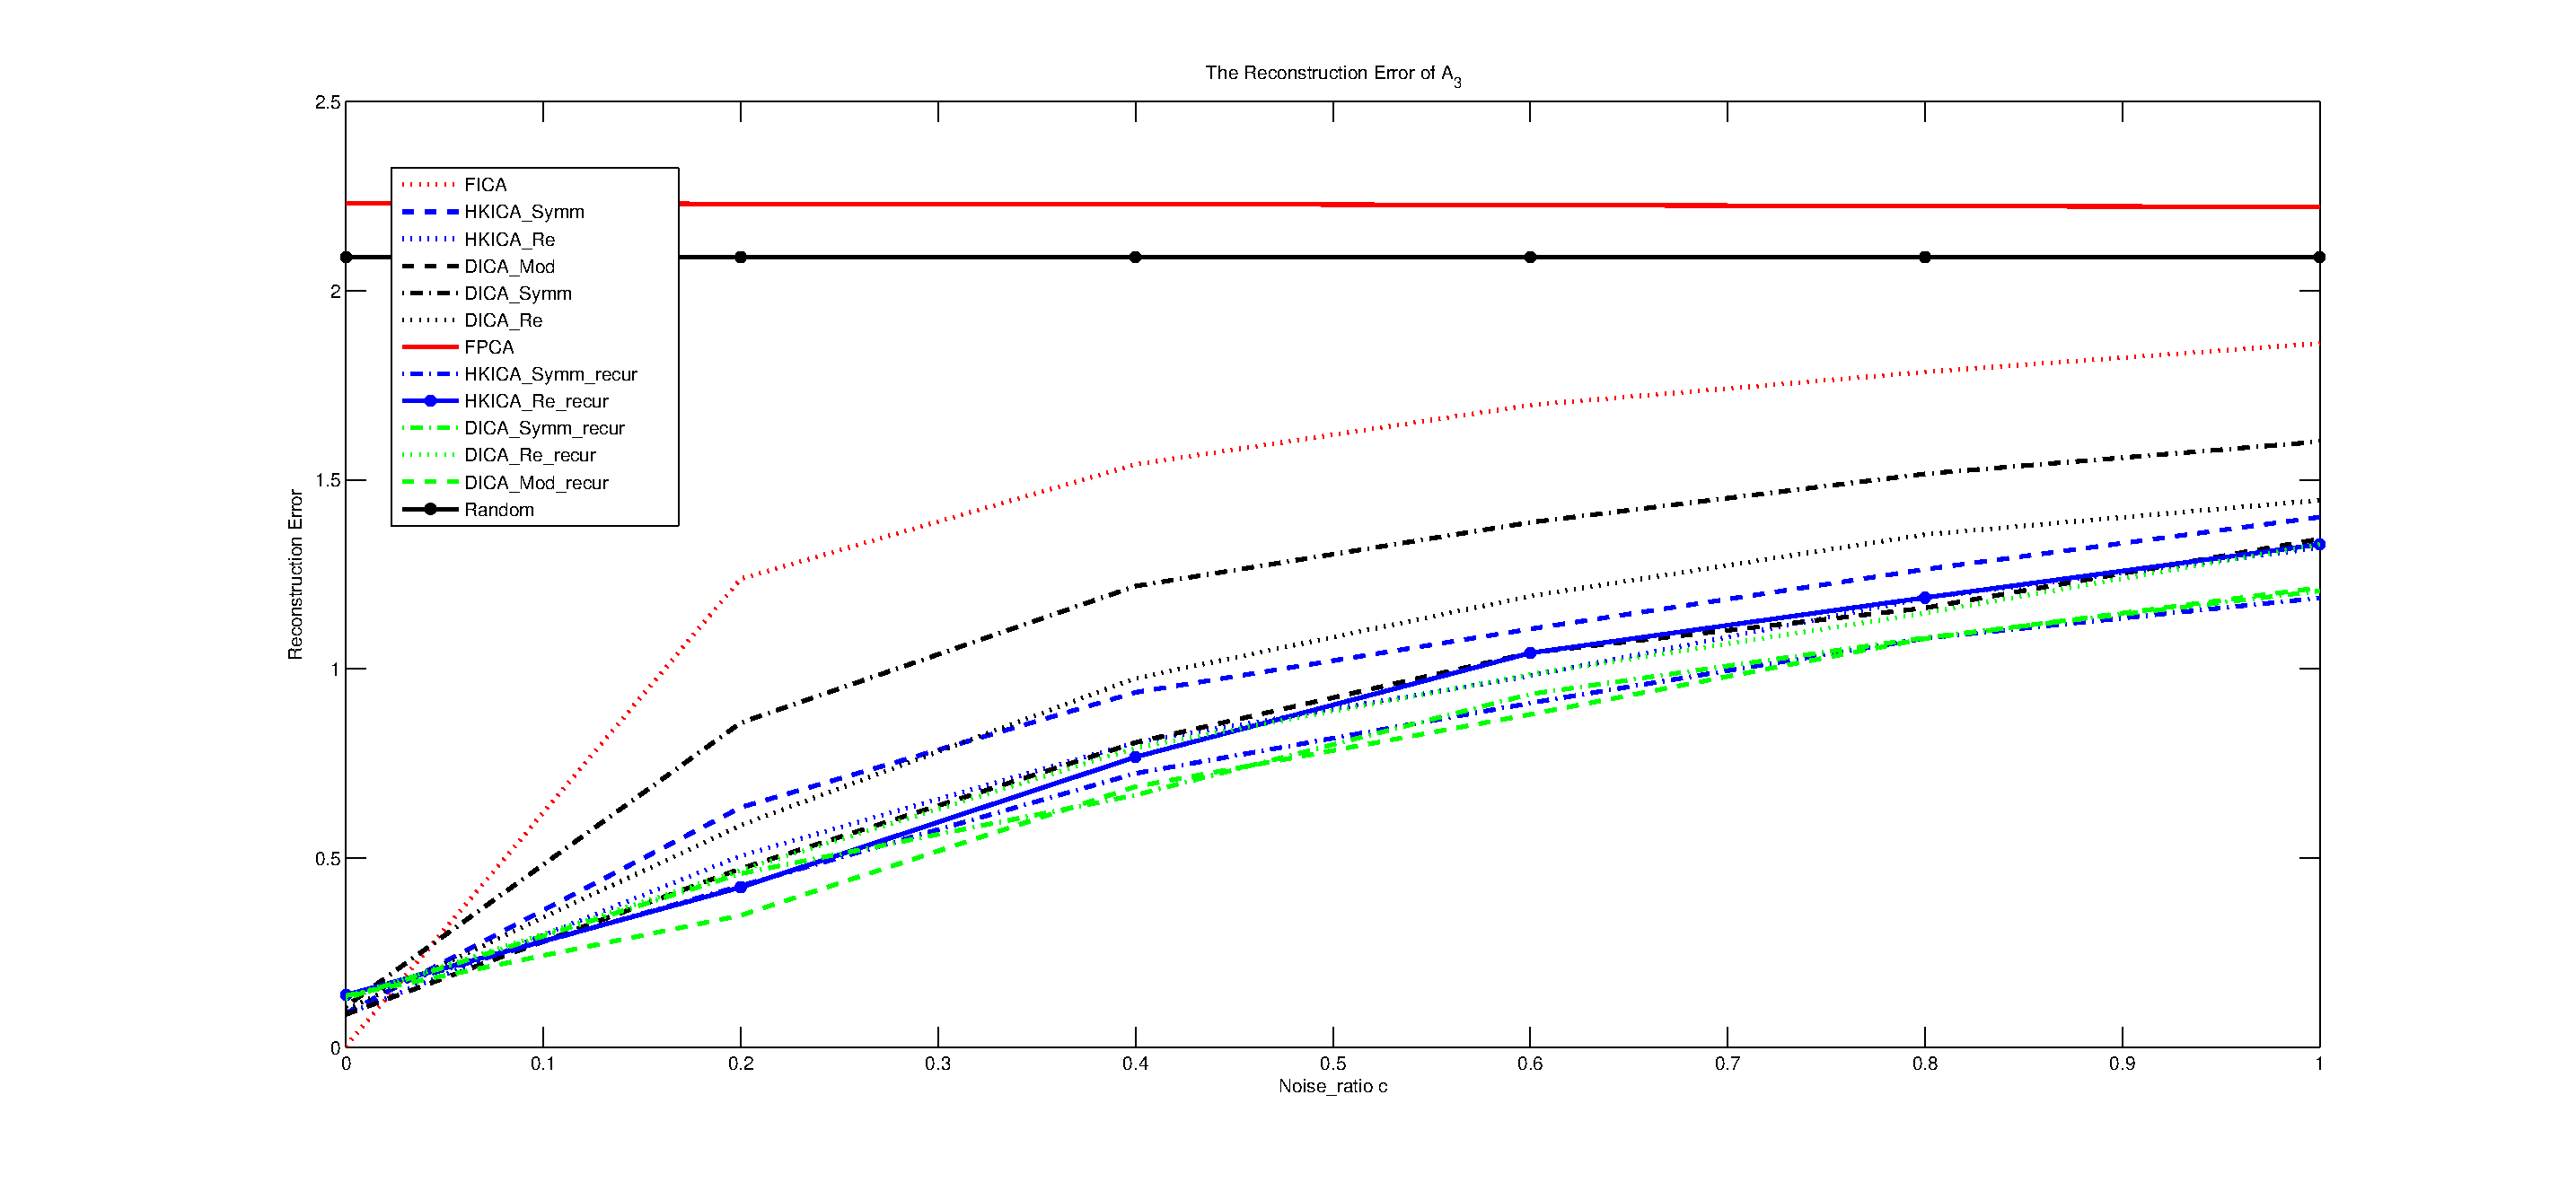
\includegraphics[height = 0.42\textheight]{error3}\\
	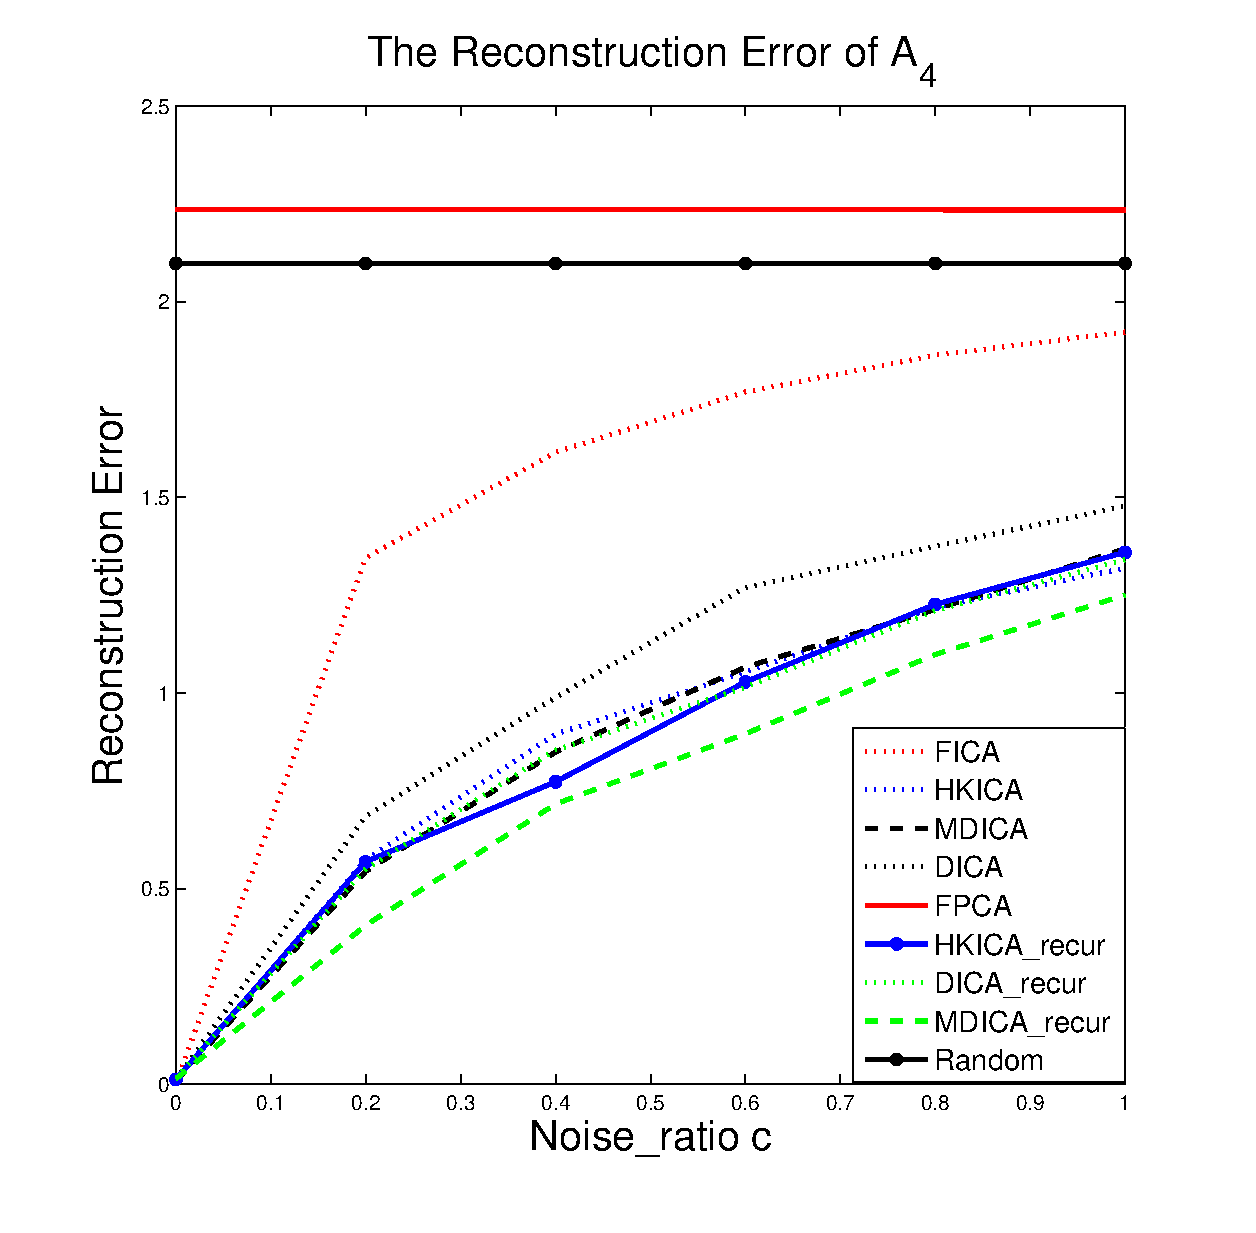
\includegraphics[height = 0.42\textheight]{error4}
\end{multicols}
}
}

\frame{ \frametitle{Simulation resutls} 
\bi
	\item Moment methods are more robust to high-coherence mixing matrices and Gaussian noise;
	\item We don't really observe improvement of DICA from HKICA in the experiments: estimation error explodes;
	\item MDICA works best, but this method only has weak theoretical guarantee;
	\item The recursive idea seems not always helpful: theoretically it only helps in the eigen-decomposition step.
\ei
} 


\frame{ \frametitle{References}
\tiny
\bibliographystyle{abbrvnat}
\bibliography{DICA}
}


\frame{ \frametitle{\,}
\begin{center}
{\huge Thank you !}
\par\end{center}{\huge \par}
\begin{center}
{\huge Questions?}
\par\end{center}{\huge \par}
} 
\end{document}
